\section{等值线图}
\label{sec:contour}
SAC中\nameref{cmd:spectrogram}等命令可以生成IXYZ数据(即3D数据),这种数据需要
用等值线图来展示。\nameref{cmd:contour}命令用于等值线,\nameref{cmd:zcolors}、
\nameref{cmd:zlabels}、\nameref{cmd:zlevels}、\nameref{cmd:zlines}、\nameref{cmd:zticks}
分别用于控制等值线的颜色、标签、间距、线型以及刻度。

下面的例子中,读入了XYZ文件contourdata,从头段中找出Z数据的范围。
选择等值线范围为700km到1150km,增量为25km。选择包括四种线型的线型表,
其中第一个为实线。这个列表将每四条等值线重复一次。然后给等值线图起了个名字,最后绘制出来:
\begin{SACCode}
SAC> r ./contourdata 
SAC> lh iftype depmin depmax
  
  FILE: ./contourdata - 1
 -------------------
       IFTYPE = GENERAL XYZ (3-D) FILE
       DEPMIN = 6.977119e+02
       DEPMAX = 1.154419e+03
SAC> zlevels range 700 1150 increment 25
SAC> zlines list 1 2 3 4
SAC> title 'Katmai topography from survey data [inc = 25 km]'
SAC> contour
\end{SACCode}

\begin{figure}[H]
\centering
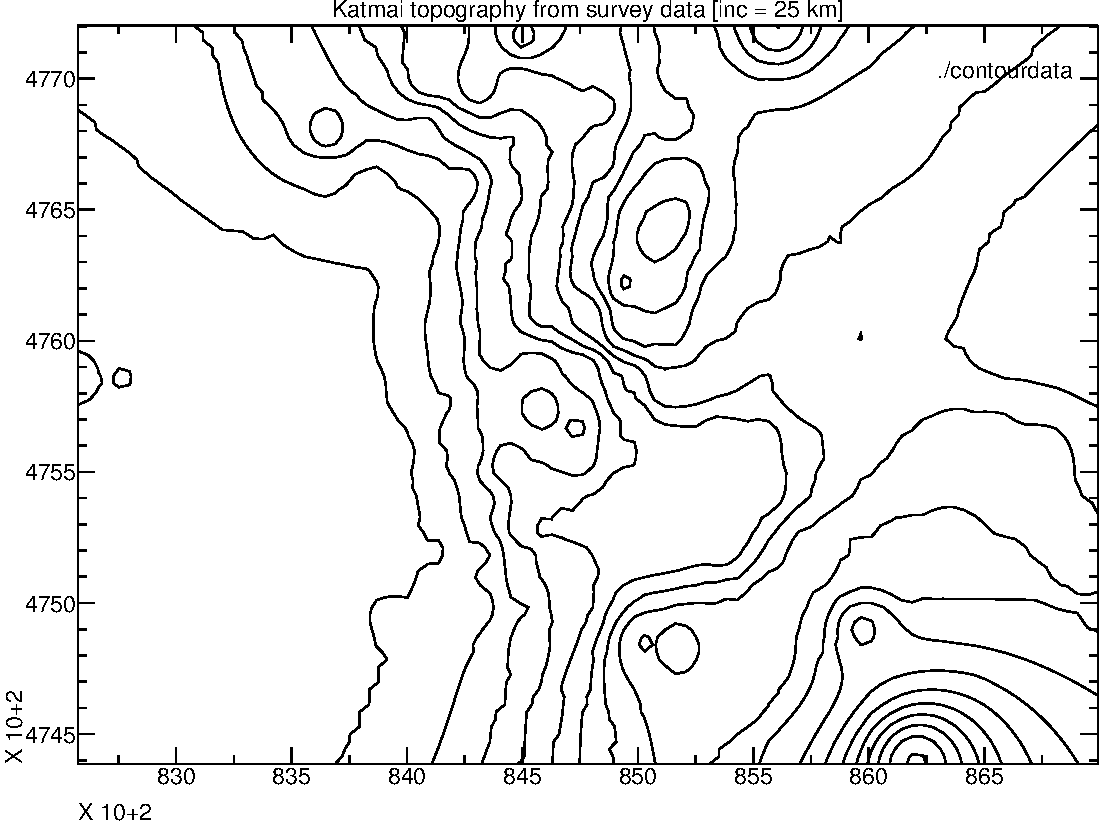
\includegraphics[width=0.9\textwidth]{contour1}
\caption{contour绘制等值线I}
\end{figure}

下面的例子中,使用同样的文件,但是显示选项不同。每四条等值线有一个整数标签。
每条等值线之间都有一个指向向下的箭头。所有等值线为实线型:
\begin{SACCode}
SAC> r ./contourdata 
SAC> zlevels range 700 1150 increment 25
SAC> zlabels on list int off off off
SAC> zticks on direction down
SAC> zlines list 1
SAC> title 'Katmai topography from survey data [labels and ticks]'
SAC> contour
\end{SACCode}

\begin{figure}[H]
\centering
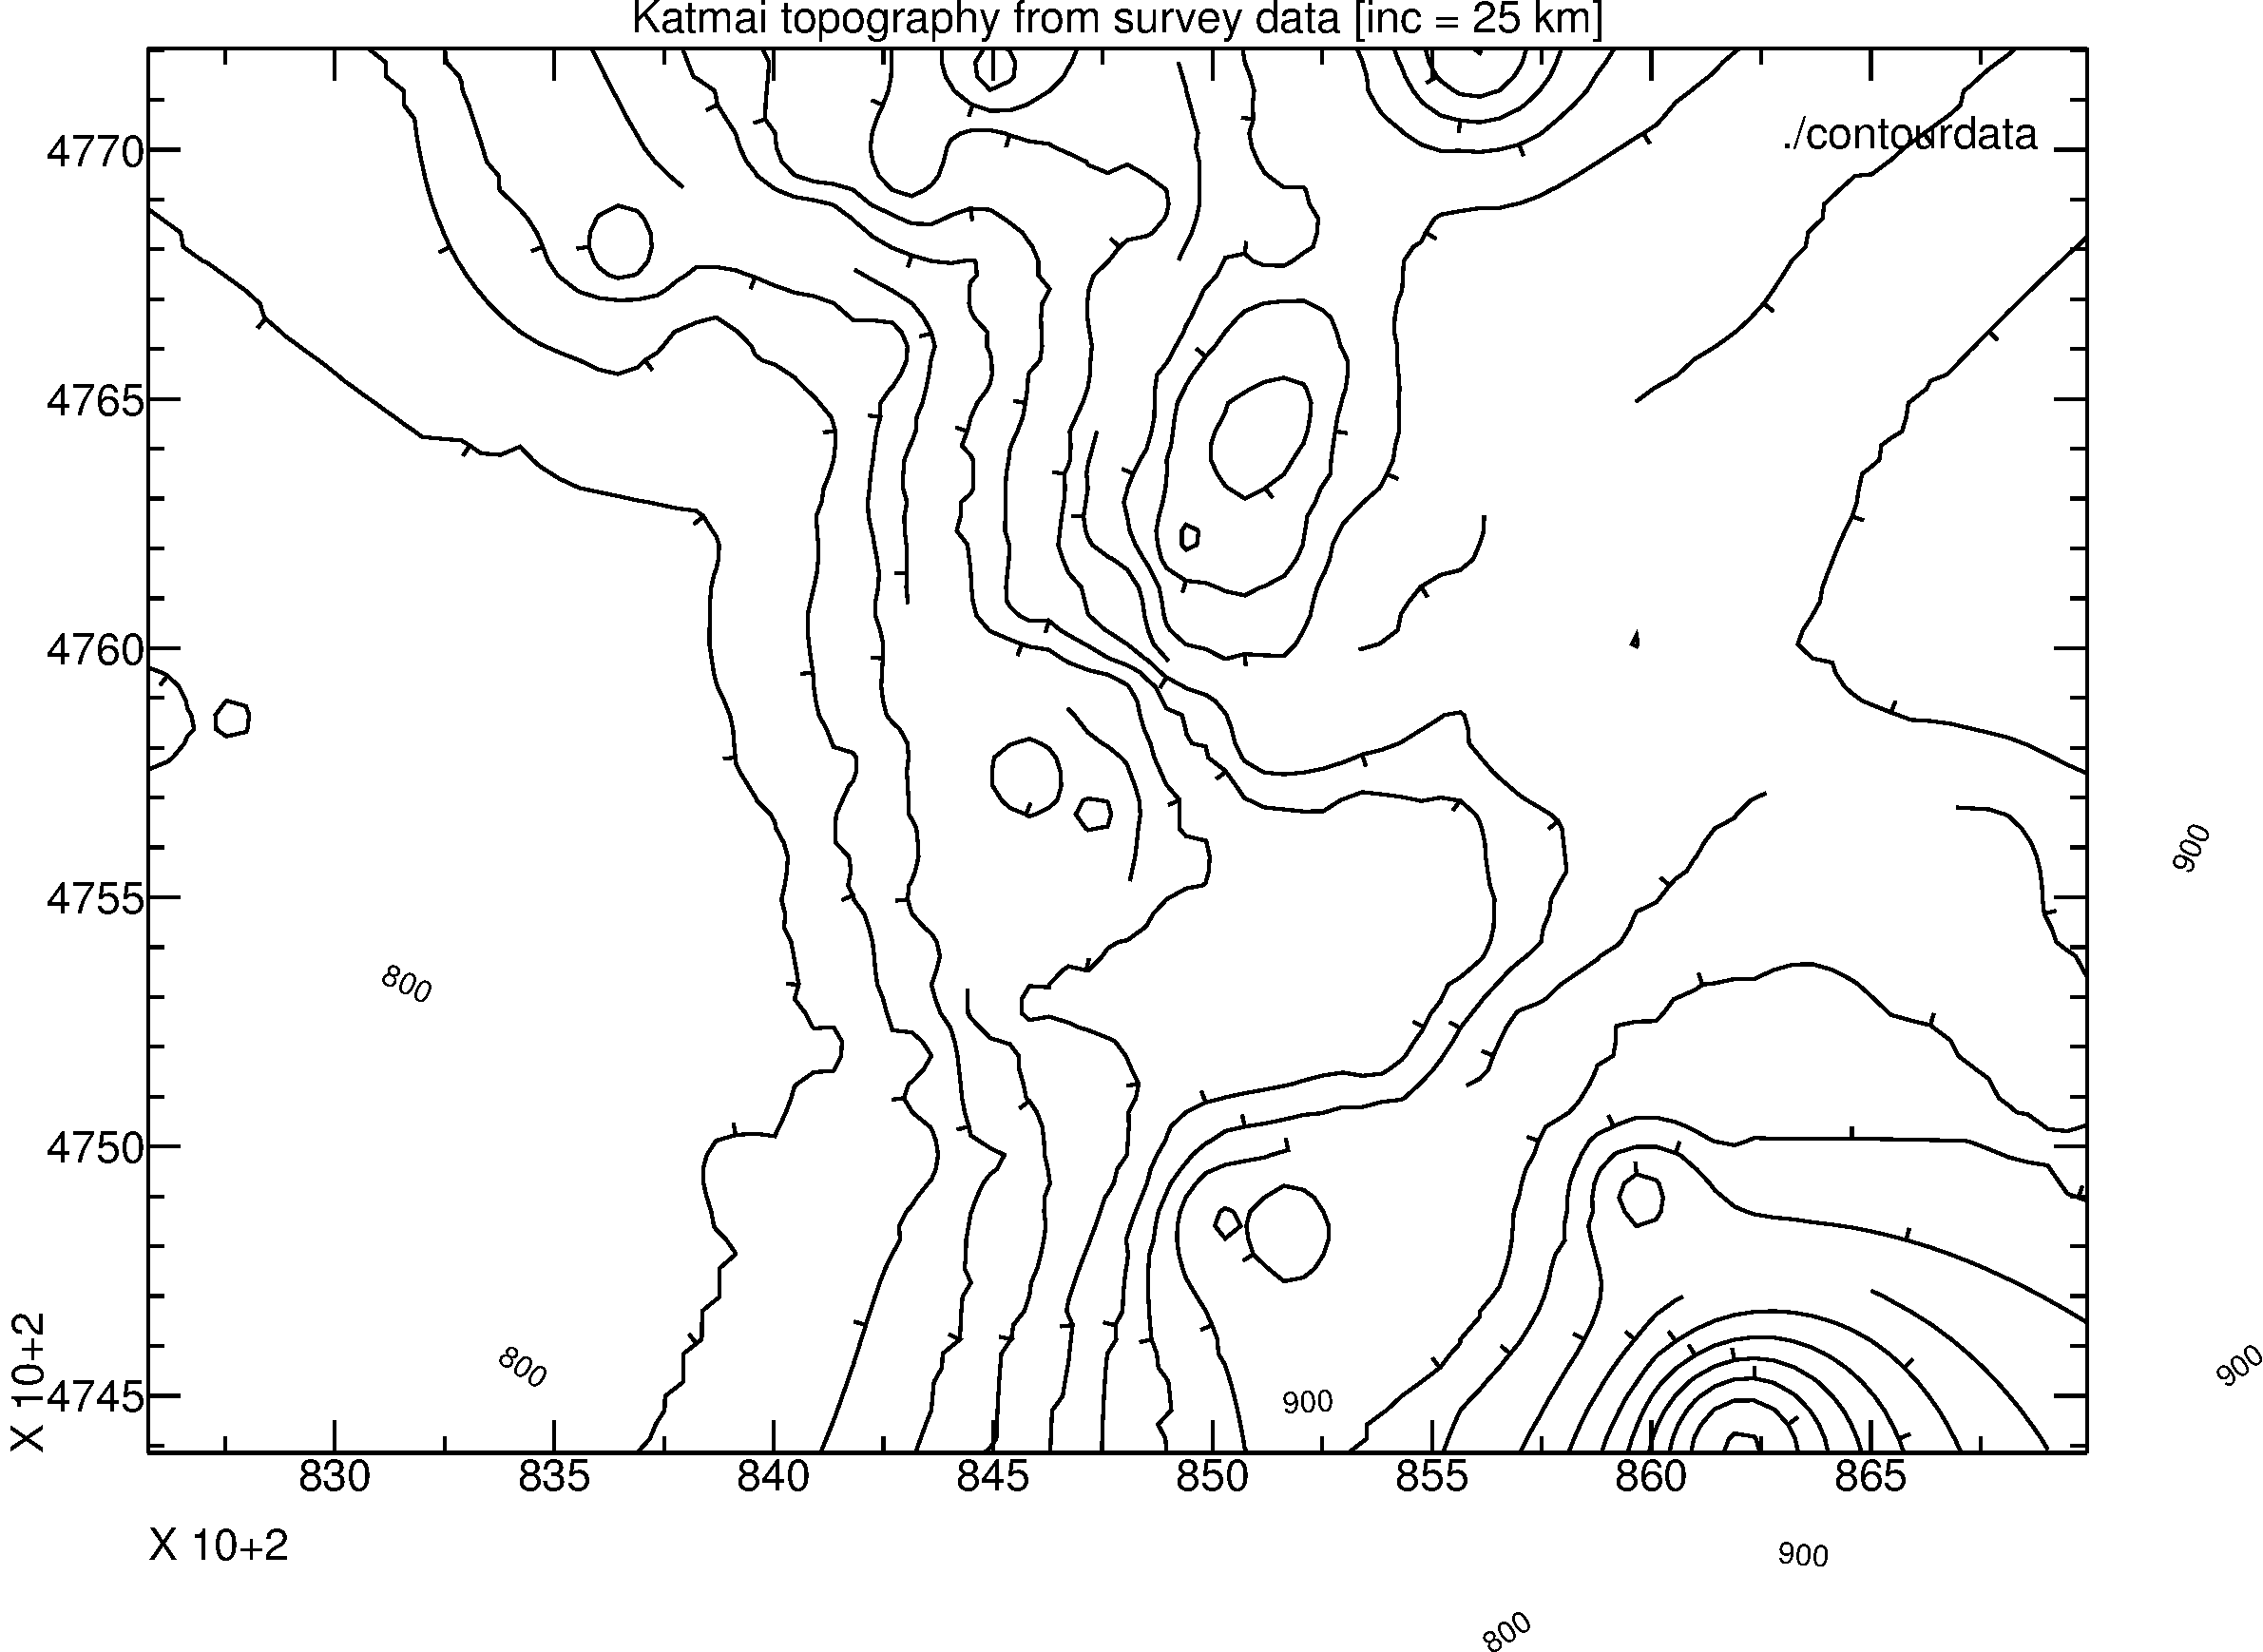
\includegraphics[width=0.9\textwidth]{contour2}
\caption{contour绘制等值线图II}
\end{figure}
